\section{واحد کنترل (\lr{Control Unit})}
واحد کنترل مدار را به صورت یک ماشین حالت متناهی (\lr{FSM}) با ۴ حالت پیاده‌سازی کردیم. وضعیت فعلی در یک ثبات ۲ بیتی ذخیره می‌شود. انتقال بین حالت‌ها و وظیفه‌ی هرکدام به این صورت می‌باشد:
\begin{itemize}
    \item \textbf{\lr{idle (00)}:} مدار در وضعیت پیش‌فرض در این حالت قرار دارد. تا زمانی که سیگنال \lr{\code{Start}} صفر باشد، در همین حالت می‌مانیم و به محض اینکه \lr{\code{Start = 1}} شود، به حالت \lr{load} منتقل می‌شویم.
    \item \textbf{\lr{load (01)}:} این حالت تنها یک چرخه طول می‌کشد. در اینجا سیگنال \lr{\code{ld}} فعال شده تا داده‌های اولیه در ثبات‌های مسیر داده بارگذاری شوند و شمارنده نیز مقداردهی اولیه (مقدار ۱) می‌شود. سپس بدون شرط به حالت \lr{calc} می‌رویم.
    \item \textbf{\lr{calc (10)}:} مدار به مدت ۳۲ چرخه در این حالت باقی می‌ماند تا واحدهای ضرب و تقسیم، محاسبات خود را انجام دهند. در این حالت سیگنال \lr{\code{WE}} فعال است (این سیگنال به عنوان ورودی در واحدهای \lr{mul} و \lr{div} استفاده شده) و مقدار شمارنده افزایش می‌یابد. با بررسی بیت پنجم خروجی شمارنده (توسط \lr{Splitter})، به محض رسیدن به عدد ۳۲، محاسبات پایان یافته و به حالت \lr{done} منتقل می‌شویم.
    \item \textbf{\lr{done (11)}:} در این حالت سیگنال خروجی \lr{\code{Done}} برابر با ۱ می‌شود که نشان‌دهنده‌ی آماده بودن نتایج در خروجی مدار است. ماشین در این حالت متوقف می‌ماند تا مجدداً سیگنال \lr{\code{Start = 1}} دریافت شود که در این صورت به طور مستقیم به حالت \lr{load} می‌رود.
\end{itemize}
برای محاسبه‌ی حالت بعدی این \lr{FSM}، به سادگی از دو مالتی‌پلکسر ۴ به ۱ استفاده شده که پایه‌های انتخاب (\lr{Select}) آن‌ها به خروجی ثبات حالت فعلی وصل شده.
\begin{figure}[H]
    \centering
    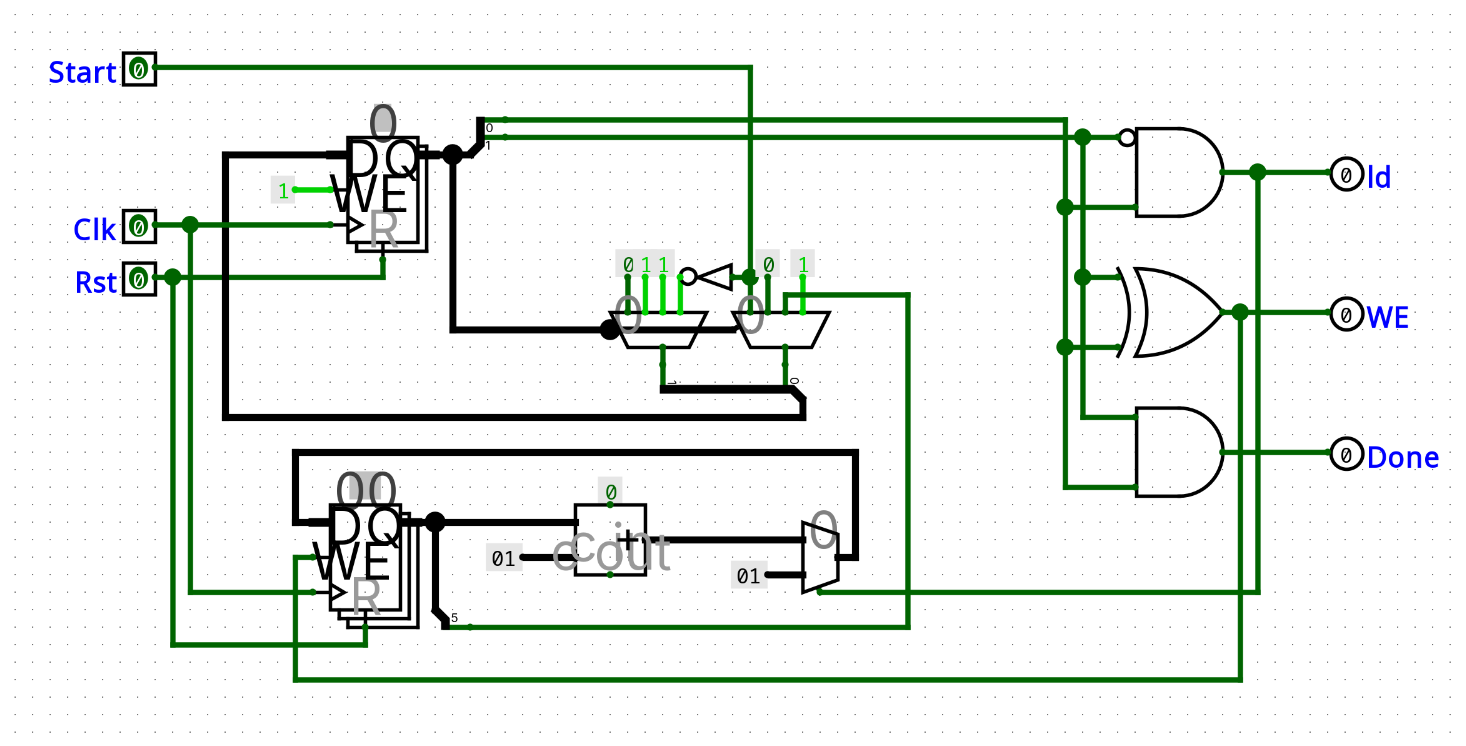
\includegraphics[width=0.7\textwidth]{assets/ctrl_unit.png}
    \caption{واحد کنترل (\lr{Control Unit})}
\end{figure}

\section{مسیر داده (\lr{Datapath})}

\subsection{ضرب‌کننده‌ی ترتیبی (\lr{Sequential Multiplier})}
در ضرب‌کننده از یک ثبات ۶۴ بیتی برای نگه داشتن حاصل ضرب استفاده کردیم. در چرخه‌ی ابتدایی (حالت \lr{load})، داده‌ی اولیه ورودی \lr{\code{B}} (که \lr{Zero-Extend} شده است) درون این ثبات قرار می‌گیرد.
در هر یک از ۳۲ چرخه‌ی محاسبه، مدار باید تصمیم بگیرد که آیا نیاز به جمع کردن مقادیر هست یا خیر؛ برای این منظور، بیت کم‌ارزش ثبات (\lr{\code{Q[0]}}) بررسی می‌شود. اگر این بیت ۱ باشد، ورودی \lr{\code{A}} با نیمه بالایی ثبات (\lr{\code{Q[63:32]}}) درون یک جمع‌کننده ۳۲ بیتی جمع می‌شود. از یک مالتی‌پلکسر با پایه‌ی انتخاب \lr{\code{{Q[0]'}}} استفاده کردیم تا تعیین کنیم خروجی جمع‌کننده انتخاب شود یا همان مقدار قبلی.
برای عملیات شیفت به راست، خروجی ۳۳ بیتیِ جمع‌کننده (شامل \lr{Carry}) در کنار بیت‌های ۱ تا ۳۱ خروجی ثبات قرار گرفته و به کمک \lr{Splitter} با هم تجمیع می‌شوند تا به ورودی ثبات متصل گردند. این جابه‌جایی در سیم‌کشی، یک واحد شیفت به راست منطقی را در هر چرخه روی داده‌ها اعمال می‌کند.
\begin{figure}[H]
    \centering
    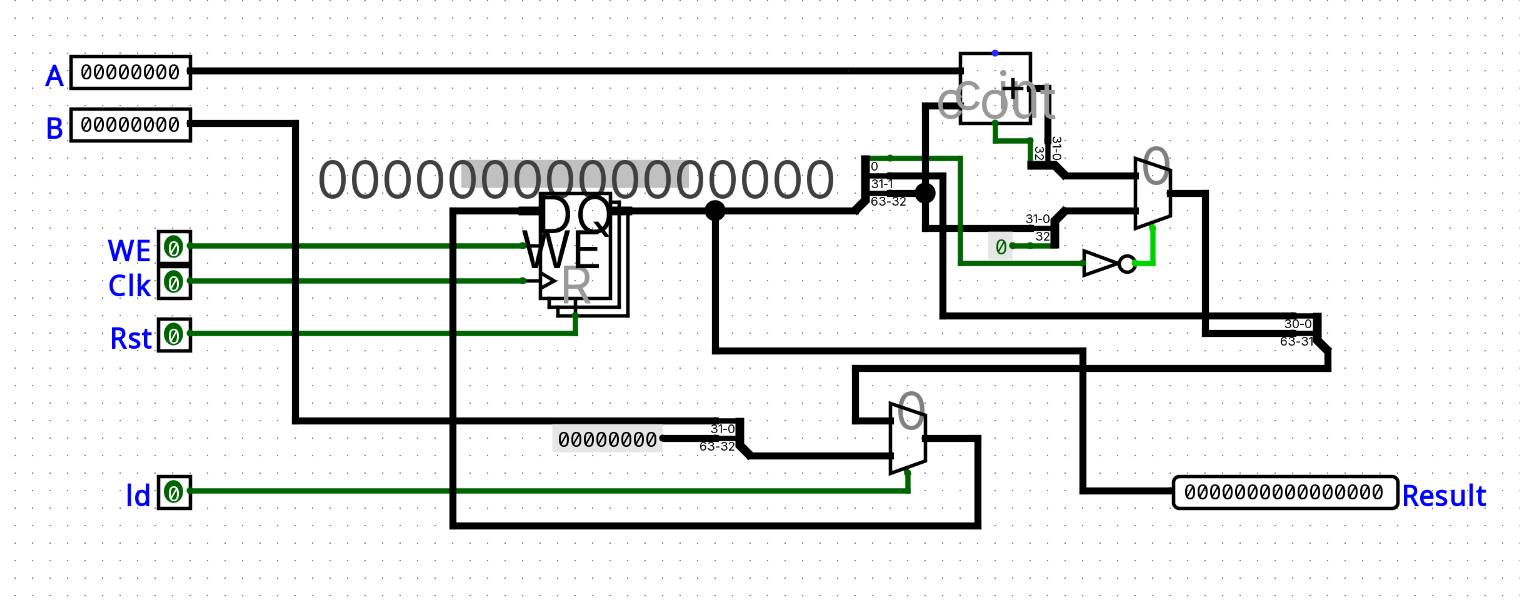
\includegraphics[width=1.0\textwidth]{assets/mul.png}
    \caption{پیمانه‌ی ضرب‌کننده ترتیبی}
\end{figure}

\subsection{تقسیم‌کننده‌ی ترتیبی (\lr{Sequential Divider})}
ساختار واحد تقسیم‌کننده تا حد زیادی شبیه ضرب‌کننده است، با این تفاوت که به جای شیفت به راست، با کنار گذاشتن \lr{MSB} و جابجا کردن بیت‌ها توسط \lr{Splitter}، عملیات شیفت به چپ را پیاده‌سازی کردیم.
برای عمل تفریق در هر چرخه، ورودی \lr{\code{B}} از گیت‌های \code{NOT} عبور کرده و با استفاده از یک جمع‌کننده (با ورودی ثابت \lr{\code{c\_in = 1}}) از ۳۲ بیت بالایی ثبات (\lr{Remainder}) کسر می‌شود.
برای پیاده‌سازی منطق تقسیم جبرانی (\lr{Restoring})، از بیت \lr{\code{c\_out}} جمع‌کننده استفاده شده است. اگر نتیجه‌ی تفریق منفی شود (\lr{\code{c\_out}} صفر باشد)، به این معنی است که نباید تفریق انجام شود، پس یک مالتی‌پلکسر مقدار قبلی را برمی‌گرداند تا عمل تفریق را جبران کند. اگر نتیجه مثبت شود، تفریق تایید شده و علاوه بر ذخیره‌ی مقدار جدید، بیت \lr{\code{c\_out}} به عنوان کم‌ارزش‌ترین بیت (\lr{LSB}) در جایگاه خارج‌قسمت ثبت می‌شود.

\begin{figure}[H]
    \centering
    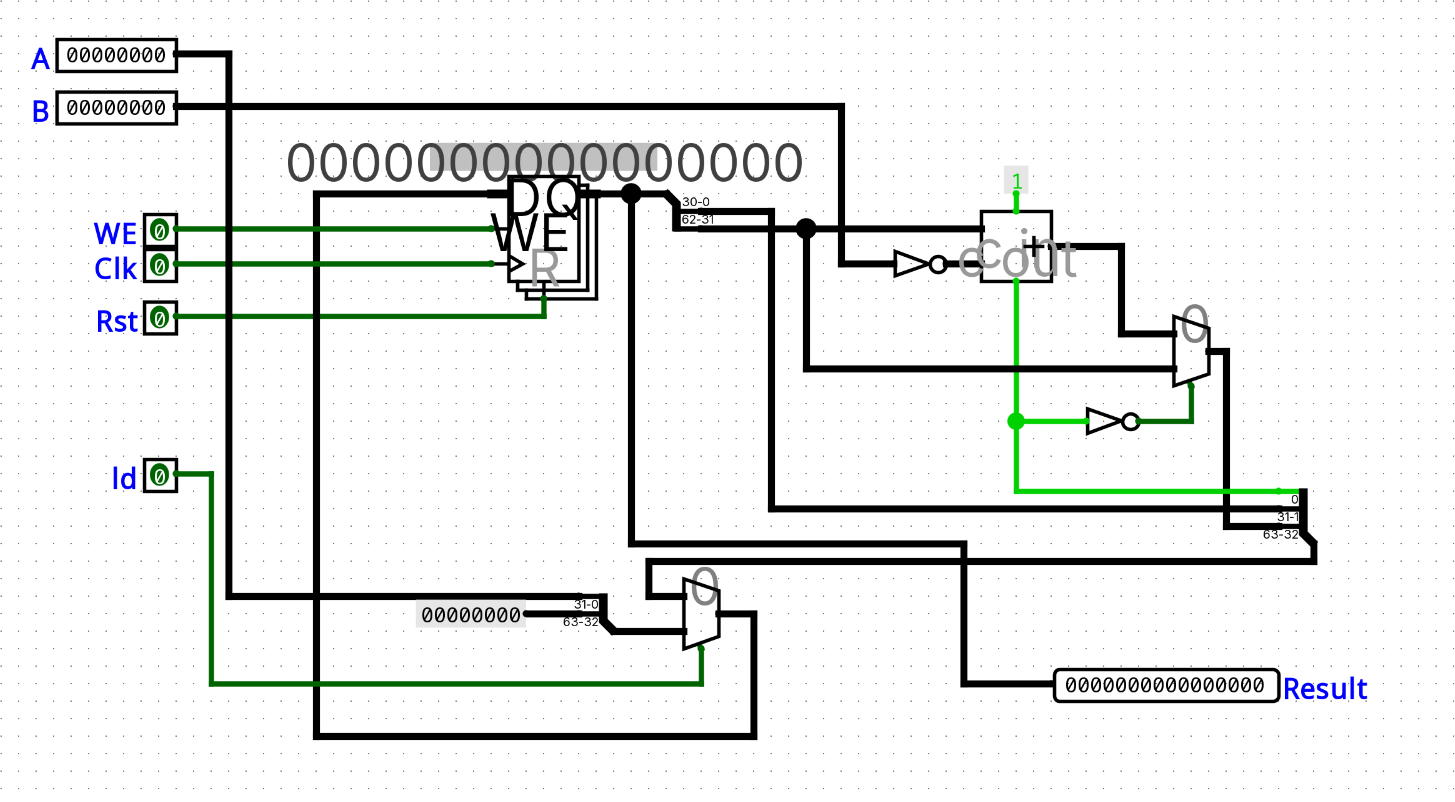
\includegraphics[width=1.0\textwidth]{assets/div.png}
    \caption{پیمانه‌ی تقسیم‌کننده ترتیبی با روش جبرانی}
\end{figure}

\section{مدار نهایی}
در نهایت، واحد کنترل، ضرب‌کننده و تقسیم‌کننده را درون یک مدار واحد ترکیب کردیم. ورودی‌های \lr{\code{A}} و \lr{\code{B}} همواره به صورت موازی به هر دو واحد \lr{Mul} و \lr{Div} متصل هستند و با شروع عملیات، هر دو مدار به طور همزمان ۳۲ چرخه محاسباتی خود را طی می‌کنند.
در بخش خروجی، با استفاده از یک مالتی‌پلکسر ۶۴ بیتی که پایه‌ی \lr{Select} آن به سیگنال ورودی \lr{\code{Divide}} متصل است، نتیجه‌ی مدار خواسته شده انتخاب می‌شود. در انتها خروجی این مالتی‌پلکسر توسط یک \lr{Splitter} به دو بخش مجزای ۳۲ بیتی \lr{\code{Result\_Lo}} و \lr{\code{Result\_Hi}} تفکیک می‌گردد.

\begin{figure}[H]
    \centering
    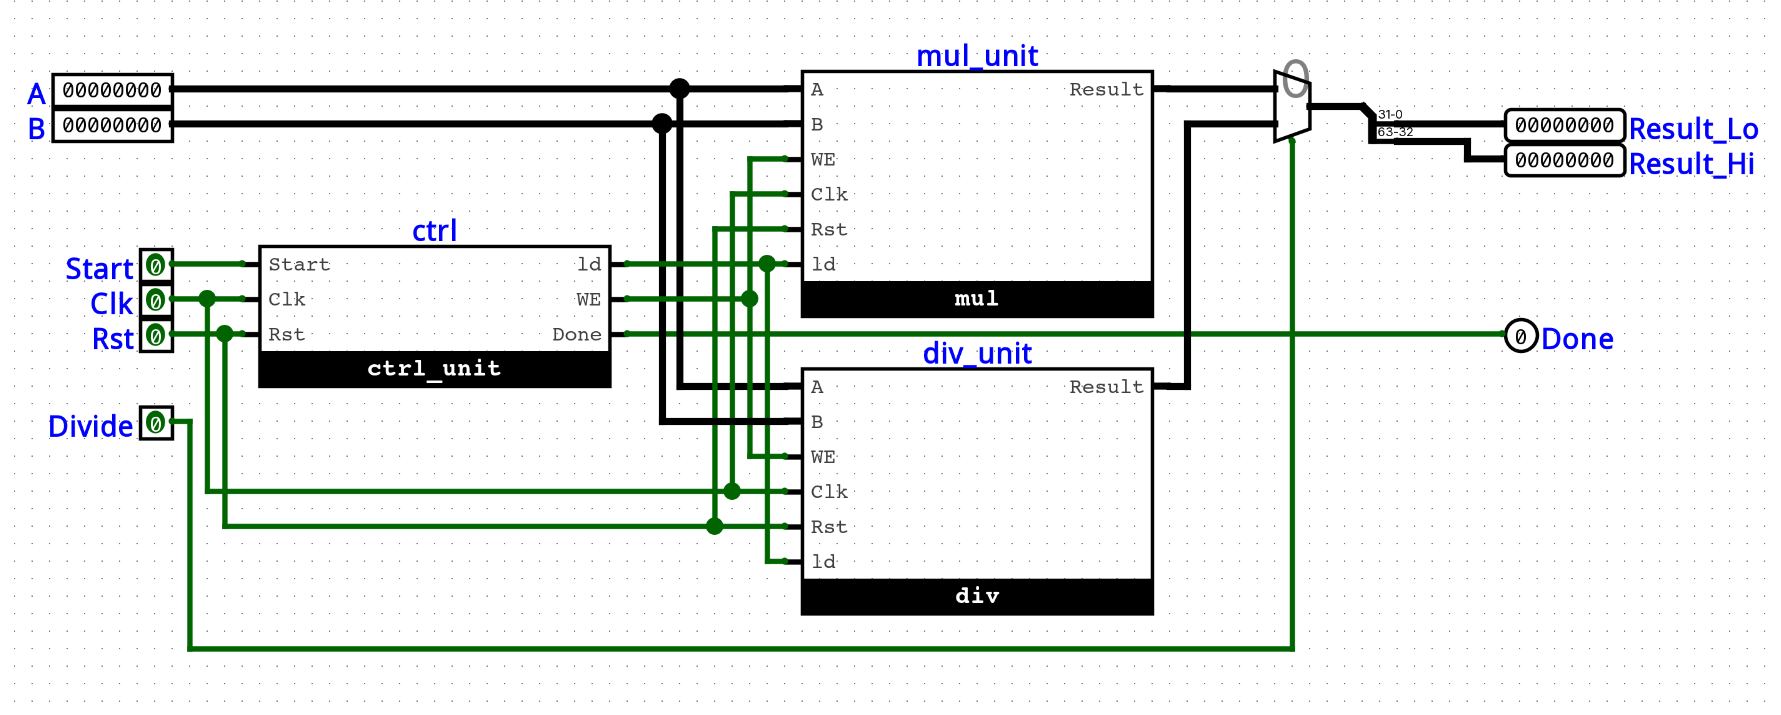
\includegraphics[width=1.0\textwidth]{assets/main.png}
    \caption{مدار اصلی ضرب/تقسیم‌کننده ترتیبی}
\end{figure}

\pagebreak

\section{اجرای آزمون}

\begin{figure}[H]
    \centering
    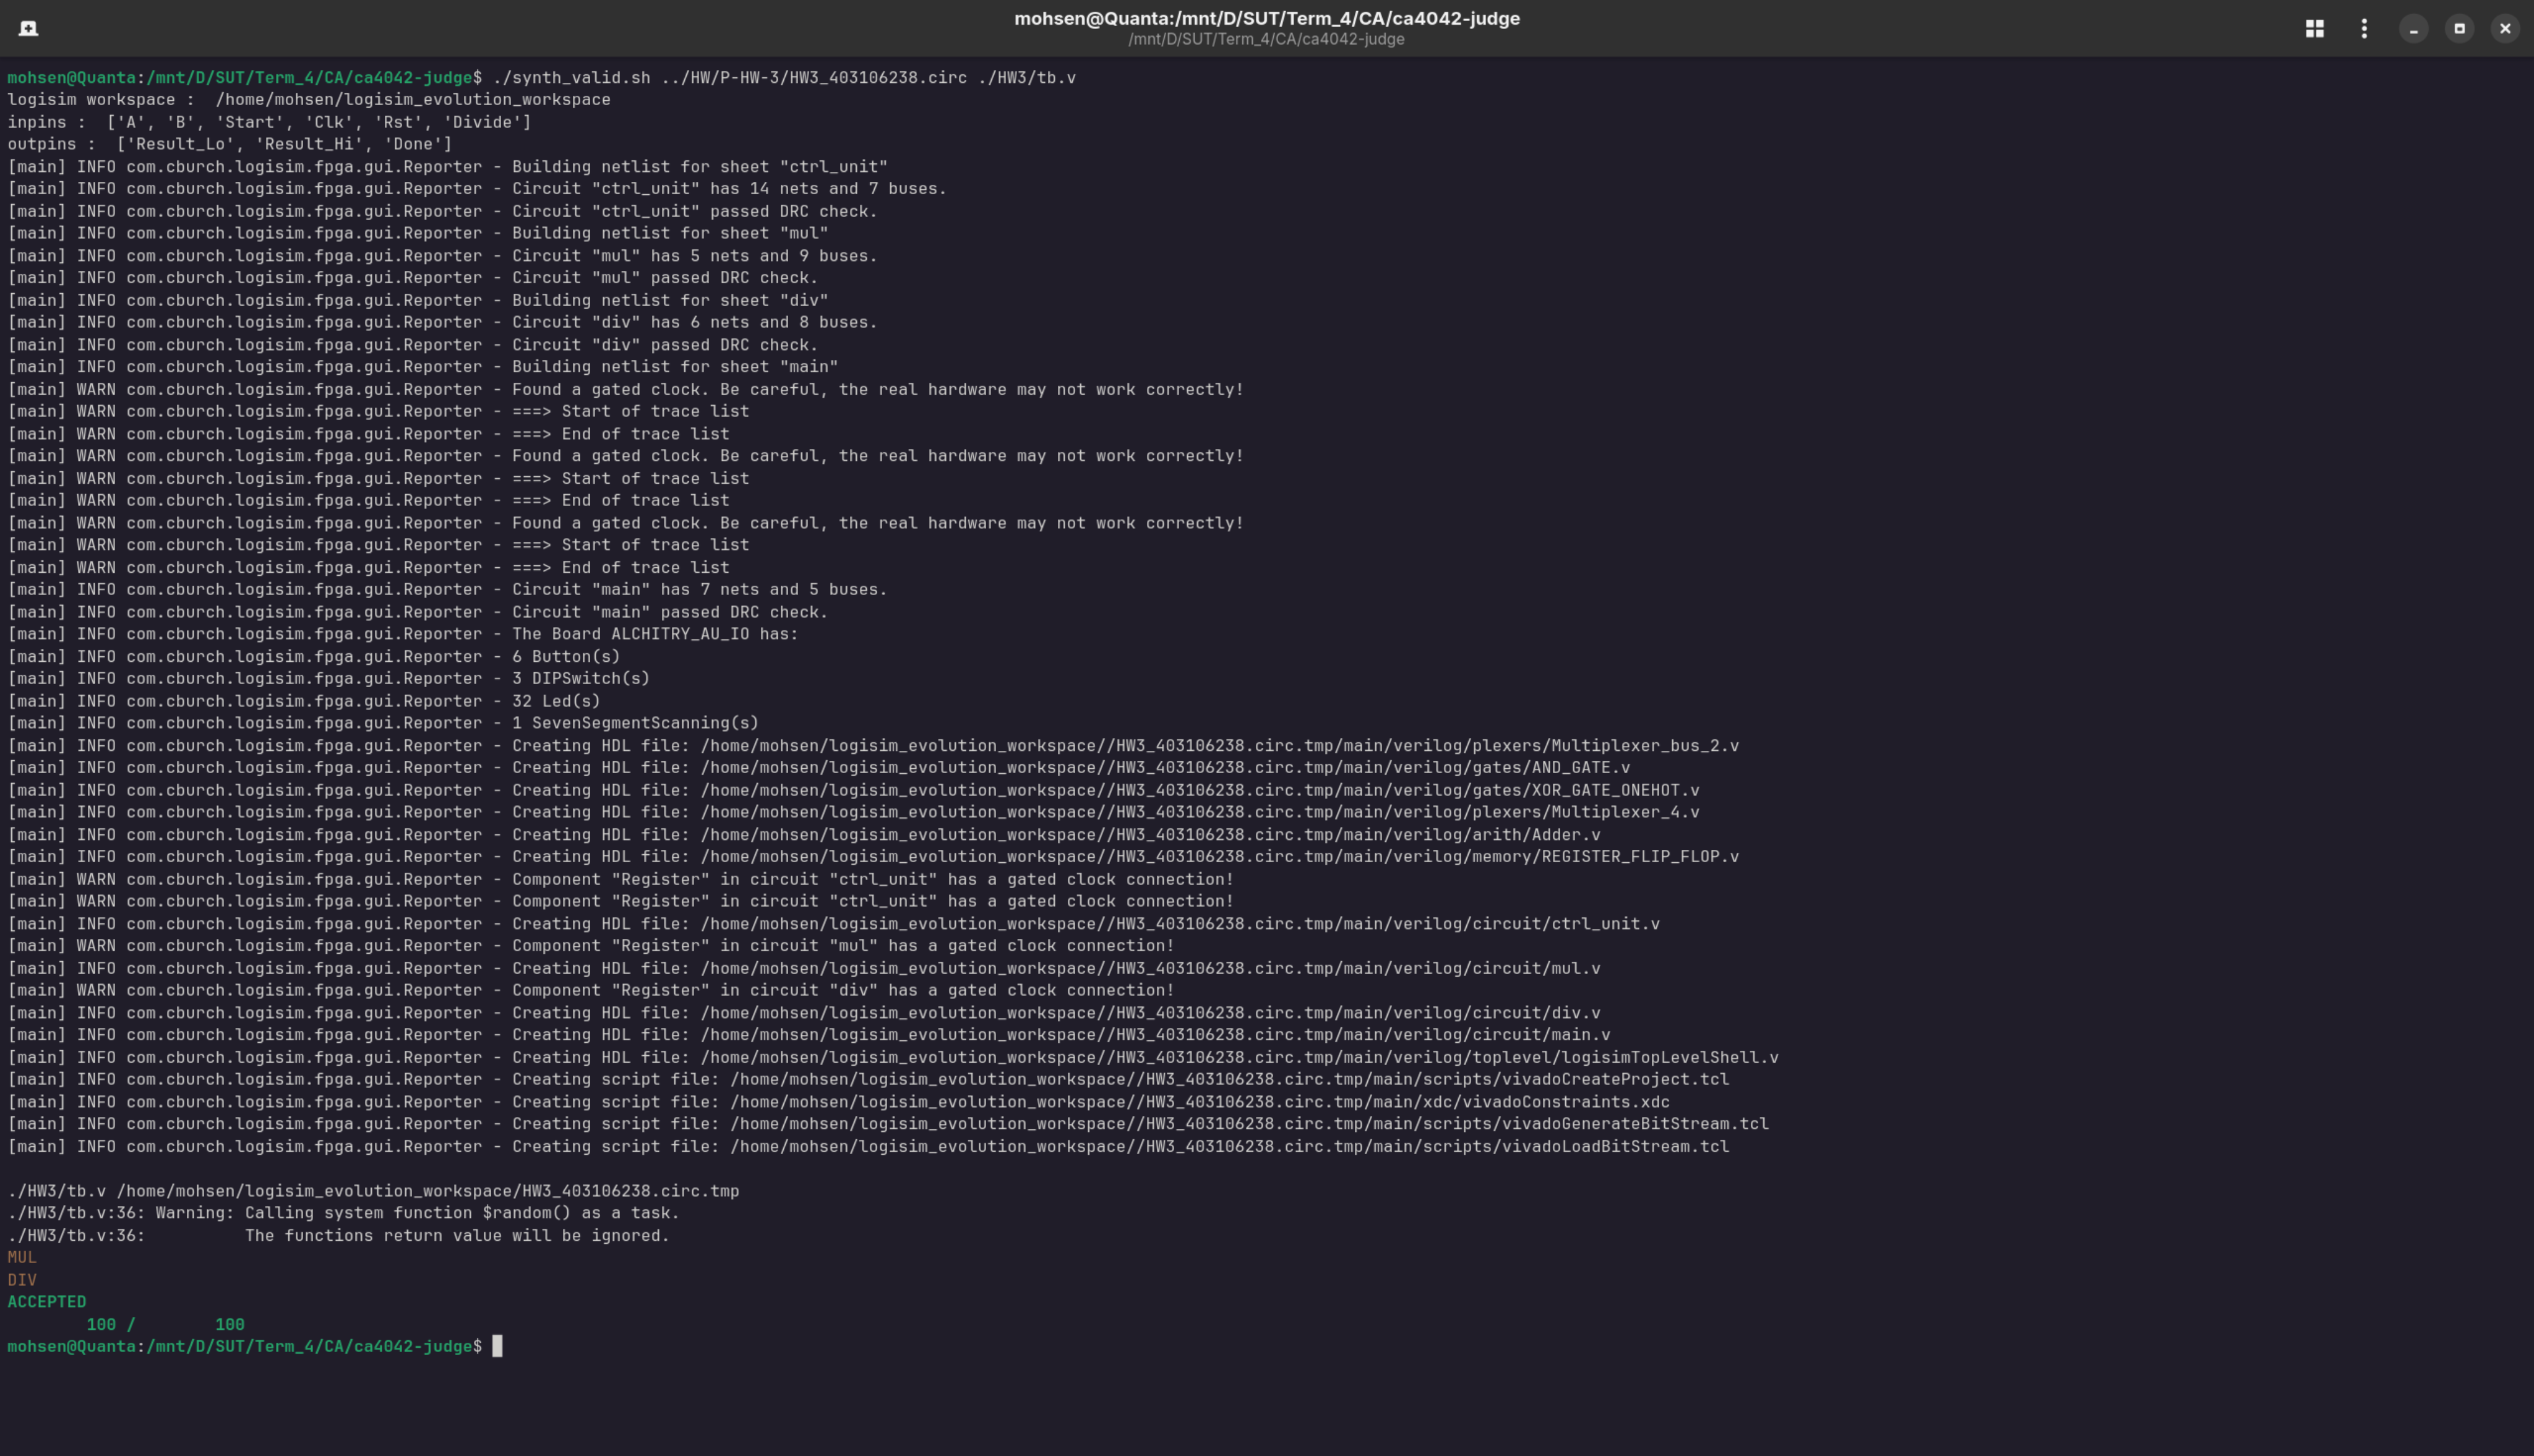
\includegraphics[width=1.0\textwidth]{assets/test.png}
    \caption{تست مدار طراحی شده}
\end{figure}